\chapter{Método de Floquet-Magnus aplicado al cálculo de Hamiltonianos efectivos}\label{cap:10}

En esta sección se desarrolla un método para describir la dinámica cuántica del electrón en la red, bajo la influencia de campos externos rápidamente oscilantes. Se utilizan métodos perturbativos, en especifico, la ya estudiada expansión de Floquet-Magnus. Se calculan los Hamiltonianos efectivos y sus respectivas energías y autofunciones para los casos de perturbación lineal y no lineal dependientes del tiempo. 

La dinámica de una partícula cuántica esta descrita por la ecuación de Schrödinger:

\begin{equation}\label{eq:10.1}
    i\hbar\frac{\partial \Psi(x,t)}{\partial t}=H(x,t)\Psi(x,t)
\end{equation}

Donde se observa que el Hamiltoniano del electrón es una función dependiente del tiempo. Se conoce la forma de las soluciones a esta ecuación diferencial gracias a la Teoría de Floquet, y se usa la expansión de Floquet-Magnus, la cual se desarrolló en el capítulo \ref{cap:8}. Se va a aplicar este método sobre Hamiltonianos que tienen la forma general presentada en la siguiente ecuación: 

\begin{equation}\label{eq:10.2}
    H(x,t)=-2A\cos(ak)+V_1(x)+V_2(x,t)
\end{equation}

Este es el hamiltoniano para un electrón en una red de \textit{Enlace Fuerte}, a la cual se ha agregado una perturbación independiente del tiempo $V_1(x)$ y una perturbación rápidamente oscilante de frecuencia $\omega \gg \omega_0$, donde $\omega_0$ es la frecuencia de las oscilaciones de Bloch.

La solución a la ecuación de Schrödinger para el Hamiltoniano de estudio fue dada por Floquet y tiene la forma:

\begin{equation}\label{eq:10.3}
    \Psi(\rho,t)=P(t)e^{-i\overline{H}t}\psi(\rho)
\end{equation}

%\begin{equation}\label{eq:10.4}
 %   \psi(\rho,t)=\sum^{\infty}_{n=-\infty} b_n e^{i(an+\lambda)\rho}
%\end{equation}

Las fórmulas recursivas de Floquet-Magnus permiten hallar el hamiltoniano efectivo para el sistema que se desea estudiar. Las fórmulas están por: 

\begin{equation}\label{eq:10.5}
    G^{(k)}=\frac{1}{T}\int^{T}_{0}\{ H(t')P^{(k-1)}(t')-\sum^{k-1}_{j=1} P^{(j)}G^{(k-j)}\}dt'
\end{equation}

\begin{equation}\label{eq:10.6}
    P^{(k)}=-i\int^{t}_{0}\{ H(t')P^{(k-1)}(t')-\sum^{k-1}_{j=1} P^{(j)}G^{(k-j)}-G^{(k)}\}dt'
\end{equation}

Los términos de orden cero en las ecuaciones \ref{eq:10.5} y \ref{eq:10.6} se han definido como en las ecuaciones \ref{eq:10.7} y \ref{eq:10.8}, tal y como se hizo en el capítulo \ref{cap:8}:

\begin{equation}\label{eq:10.7}
    \begin{cases}
        G^{(0)}=0\\
        P^{(0)}=1
    \end{cases}
\end{equation}

\begin{equation}\label{eq:10.8}
\begin{cases}
    G=\sum G^{(k)}\\
    P=\sum P^{(k)}
    \end{cases}
\end{equation}

Donde $\overline{H}=G$. Para este trabajo especial de grado se estudian las perturbaciones dependientes del tiempo que tienen la siguiente forma general:

\begin{equation}\label{eq:10.9}
    V_2(x,t)=V(x)\cos(\omega t)
\end{equation}

Para efectos del calculo de $P^{(k)}$ y $G^{(k)}$ se ha creado un programa en \textit{Mathematica} cuyo algoritmo permite el cálculo hasta orden $k=5$ para cualquier perturbación externa del electrón en la red. 

\section{Dinámica del electrón en la red de \textit{Tight Binding} en presencia de una perturbación lineal dependiente del tiempo }

En esta sección se estudia el caso del electrón en la red de \textit{Tight Binding}, en presencia de un potencial eléctrico externo lineal y rápidamente oscilante. El Hamiltoniano de este sistema tiene la siguiente forma:

\begin{equation}\label{eq:10.10}
    H(x,t)=2A\cos(a\rho)+\epsilon x \cos(\omega t)
\end{equation}

Haciendo uso de la expansión de Floquet-Magnus se calculan los $G^{(k)}$ hasta $k=5$ y los $P^{(k)}$ hasta $k=4$ con ayuda del programa de \textit{Mathematica} hecho especialmente para este fin. A continuación se presentan los resultados obtenidos:

\subsection{Cálculo de los $G_{(K)}$ y $P_{(k)}$}

\begin{equation}\label{eq:10.11}
    G^{(1)}=-2A\cos(ap)=H_o
\end{equation}

\begin{equation}\label{eq:10.12}
    P^{(1)}=\frac{\epsilon\sin(\omega t)}{\omega}\mathbb{I}
\end{equation}

\begin{equation}\label{eq:10.13}
    G^{2}=0
\end{equation}

\begin{equation}\label{eq:10.14}
    P^{(2)}=\frac{\epsilon\sin^2(\frac{t\omega}{2})}{\omega^2}[4iaA\sin(ap)\mathbb{I}+2\epsilon\cos^2(\frac{t\omega}{2})\frac{\partial^2}{\partial p^2}]
\end{equation}

\begin{equation}\label{eq:10.15}
    G^{(3)}=\frac{a^2A\epsilon^2\cos(ap)}{2\omega^2}\mathbb{I}
\end{equation}

\begin{equation}\label{eq:10.16}
         \begin{split}         P^{(3)}=&\frac{\epsilon^2}{12\omega^3}[3ia^2A(8\sin(\omega t)-3\sin(2\omega t))\cos(ap)\mathbb{I} +\\&+48iaA\sin^2(\frac{\omega t}{2})\sin(\omega t)\sin(ap)\frac{\partial}{\partial p}+\\&+ 2i\epsilon\sin^3(\omega t)\frac{\partial^3}{\partial p^3}]
    \end{split}
\end{equation}

\begin{equation}
  G^{(4)}=0  
\end{equation}

\begin{equation}\label{eq:10.17}
\begin{aligned}
        &P^{(4)}=\frac{\epsilon^2 \sin ^2\left(\frac{t \omega}{2}\right)}{36 \omega^4} (6 \epsilon^2  \sin ^2(t\omega) \cos^2 \left(\frac{t \omega}{2}\right)\frac{\partial^4}{\partial p^4}-\\&-72 i a^2 A \epsilon  \cos (a p) \cos
   ^2\left(\frac{t \omega}{2}\right) (3 \cos (t \omega)-4)\frac{\partial}{\partial p}+\\&+72 i a A \epsilon \sin (a p) \sin ^2(t \omega)\frac{\partial^2}{\partial p^2}-\\&-2 i a^2 A \sin (a p) (a \epsilon (14 \cos (t w)-11 \cos (2 t \omega)+33)+\\&+72 i A \sin (a p) (\cos
   (t \omega)-1))\mathbb{I})
    \end{aligned}
\end{equation}

\begin{equation}\label{eq:10.18}
    G^{(5)}=-\frac{a^4 A \epsilon^4\cos(a p)}{32 \omega^4}\mathbb{I}
\end{equation}


 Estos resultados fueron contrastados con los de Martínez et al.(2017) obteniendo exactamente las mismas expresiones para los $G$ y $P$ hasta $k=5$ \cite{martinez2017}. Al observar con detenimiento las expresiones para $G^{(k)}$ en $k=1,2,3,4,5$ se observa que es posible encontrar una solución general para cualquier  $G^{(k)}$,

\begin{equation}\label{eq:10.19}
    G^{[1]} \approx G^{(0)}+G^{(1)}=-2A\cos (a p)\mathbb{I}
\end{equation}

\begin{equation}\label{eq:10.20}
    G^{[3]} \approx G^{(0)}+G^{(1)}+G^{(2)}+G^{(3)}=-2A\cos (a p)\left(1-\frac{a^2 \epsilon^2  }{4 \omega^2}\right)\mathbb{I}
\end{equation}

\begin{equation}\label{eq:10.21}
    G^{[5]} \approx G^{(0)}+G^{(1)}+G^{(2)}+G^{(3)}+G^{(4)}+G^{(5)}=-2A\cos (a p)\left(1-\frac{a^2 \epsilon^2  }{4 \omega^2}+\frac{a^4 \epsilon^4}{64 \omega^4}\right)\mathbb{I}
\end{equation}

\begin{equation*}
    \vdots
\end{equation*}

\begin{equation}\label{eq:10.22}
    G^{[n+1]} \ \ \overrightarrow{n \rightarrow \infty} \ \
 G^{(0)}+G^{(1)}+\dots G^{n+1}=-2A\cos(a p)\mathcal{J}_0(\frac{\omega_B}{\omega})\mathbb{I}
\end{equation}

La ecuación \ref{eq:10.22} es el resultado de la convergencia de $G$ para el caso que se está estudiando, donde $\mathcal{J}_0(z)$ es la función de Bessel, definida como:

\begin{equation}\label{eq:10.23}
    \mathcal{J}_0(z)=\sum^{\infty}_{m=0}\frac{(-1)^m}{(m!)^2}(\frac{z}{2})^{2m}
\end{equation}

Este resultado coincide con los resultados de Dunlap y Kenkre \cite{Dunlap} para el electrón en campos eléctricos oscilantes. En su artículo de 1984, ellos hallaron que el electrón moviéndose en campos eléctricos oscilantes, tiene un potencial y Hamiltoniano efectivo de la forma siguiente:

\begin{equation}
    H(X,K)=H_0(X,K)\mathcal{J}_0(\omega_0/\omega)
\end{equation}

\begin{equation}
U_{eff}(X)=U(X)\mathcal{J}_0(\omega_0/\omega)    
\end{equation}

Donde $\mathcal{J}_0(\omega_0/\omega)$ es la función de Bessel a orden cero. Estas ecuaciones indican la presencia del fenómeno de \textit{Band Narrowing}. En los puntos donde se anula la función $\mathcal{J}_0$ de Bessel la banda de energía y la interacción efectiva entre el electrón y la red se anulan. Se observa además que el campo externo oscilante tiene el efecto de reducir la velocidad efectiva o de deslocalización del electrón inicialmente localizado \cite{Dunlap}.

 Se obtienen las funciones de onda del electrón según la Teoría de Floquet-Magnus:

\begin{equation}\label{eq:10.24}
\begin{split}
    \Psi(t,p)&=P(t)e^{i\overline{H}t}\psi(p)
    \\&=CP(t)e^{iE(p)t}\delta(p-p')
\end{split}
\end{equation}

Donde $\psi(p)=C\delta(p-p')$ es la autofunción generalizada de $G$ y $E(p)=-2A\cos(a p)\mathcal{J}_0(\frac{\omega_B}{\omega})$ es su autovalor generalizado. Se aproxima la $P(t)$ y $G$ hasta orden de $\omega^{-2}$:

\begin{equation}\label{eq:10.25}
    G \approx -2A\cos (a p)\mathcal{J}
\end{equation}

\begin{equation}
    \mathcal{J}=1-\frac{a^2 \epsilon^2  }{4 \omega^2}
\end{equation}

\begin{equation}\label{eq:10.26}
    P(t)=\left(1+\frac{\epsilon\sin(\omega t)}{\omega}+\frac{4iaA\epsilon\sin^2(\frac{t\omega}{2})\sin(ap)}{\omega^2}\right)\mathbb{I}+\frac{\epsilon^2}{\omega^2}\sin^2(t\omega)\frac{\partial^2}{\partial p^2}
\end{equation}
 
 Se escoge la solución:
 
 \begin{equation}\label{eq:10.27}
     \psi(p)=\frac{a}{2\pi}\sum^{\infty}_{-\infty} e^{in(p-p')a}
 \end{equation}
 
Entonces se puede calcular la posición cuadrática promedio, y se obtiene la siguiente expresión:

\begin{equation}\label{eq:10.28}
    \bra{\Psi}X^2\ket{\Psi}\approx 2A^2a^2\mathcal{J}^2(\frac{\omega_B}{\omega})t^2
\end{equation}

Se observa que por efecto de la fuerza oscilante externa, la partícula se deslocaliza de su punto de origen y no efectúa movimientos oscilatorios. Se encuentra que este resultado coincide con el estudio semiclásico que se hizo previamente de este mismo sistema, donde el electrón también resultaba no localizado.

\section{Dinámica del electrón en la red de Enlace Fuerte en presencia de una perturbación no lineal dependiente del tiempo}

En este segundo caso de estudio se trabaja con una perturbación no lineal dependiente del tiempo, en particular la tangente hiperbólica multiplicada por $\cos(\omega t)$. En este caso el Hamiltoniano tiene la siguiente forma:

\begin{equation}\label{eq:10.29}
    H(x,t)=2A\cos(a\rho)+\tanh(\alpha x)\cos(\omega t)
\end{equation}

La perturbación, cuya inhomogeneidad en el espacio tiene la forma referencial dada por la figura \ref{fig:10.1}, tiene cierta similitud con la  ya estudiada por Martínez et al. \cite{martinez2017}, donde se estudió la inhomogeneidad lineal multiplicada por una función rápidamente oscilante. La diferencia que destaca en nuestro caso, es que, a diferencia de una perturbación lineal, la tangente hiperbólica tiene límites finitos cuando se hace tender a infinito y menos infinito, característica que la hace más realista, si a sentido físico se refiere, ya que la linealidad se limita a una región del espacio finito, mientras que en las zonas alejadas del origen la tangente está acotada con pendiente casi nula, por lo que en estas zonas el electrón experimenta fuerzas despreciables.


\begin{figure}[H]
    \centering
    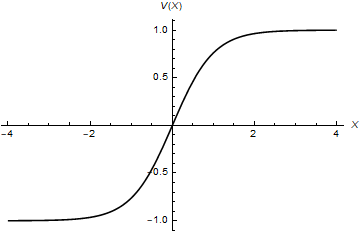
\includegraphics{imagenes/potencial_oscilante.png}
    \caption{Forma referencial de la inhomogeneidad $V(x)=\tanh(x)$}
    \label{fig:10.1}
\end{figure}

En lo sucesivo, se necesita tratar la inhomogeneidad como un operador cuántico. Se expande la $\tanh(\epsilon x)\approx \epsilon x - \gamma\frac{x^3}{3}$ y se sustituye $x$ por el operador de posición $x=i\frac{d}{d\rho}$. De esta manera el Hamiltoniano tiene la forma:

\begin{equation}\label{eq:10.30}
    \hat{H}(x,t)=2A\cos(a\rho)\mathbb{I}+i\cos(\omega t)\left( \epsilon \frac{\partial}{\partial \rho} + \frac{\gamma}{3}\frac{\partial^3}{\partial \rho^3}\right)
\end{equation}

Se hizo uso del programa en \textit{Mathematica} (ap\'endice \ref{apendice:E}) especialmente desarrollado para este cálculo y se obtuvo los siguientes resultados para los $G^k$ y $P^k$ (Esto se hizo hasta orden $k=3$ y tomando $\gamma^2=0$).

\subsection{Cálculo de $G_{(k)}$ y $P_{(k)}$}

\begin{equation}\label{eq:10.31}
    \hat{G}^{1}=-2 A \cos(a p)\mathbb{I}
\end{equation}

\begin{equation}\label{eq:10.32}
    \hat{P}^{1}=\frac{\sin(\omega t)}{3 \omega} \left(3 \epsilon \frac{\partial}{\partial \rho}+\gamma \frac{\partial^3}{\partial \rho^3}\right)
\end{equation}

\begin{equation}\label{eq:10.33}
    \hat{G}^{2}=0
\end{equation}

\begin{equation}\label{eq:10.34}
\begin{split}
     \hat{P}^{2}=&4iaA\frac{\sin (a \rho) \sin ^2\left(\frac{t \omega}{2}\right)}{\omega^2}\left( \epsilon-\frac{
    a^2 \gamma }{3}\right)\mathbb{I}+\left(\frac{4 i a^2 A \gamma }{\omega^2}\cos (a \rho) \sin ^2\left(\frac{\omega t}{2}\right)\right)\frac{\partial}{\partial \rho}+\\
    &+\frac{\sin ^2\left(\frac{t w}{2}\right)}{w^2}\left[\epsilon^2\left(1 +\cos (\omega t)\right)+4 i a A l \sin (a \rho) \right]\frac{\partial^2}{\partial \rho^2}+\frac{\epsilon \gamma \sin ^2(\omega t)}{3 \omega^4}\frac{\partial^4}{\partial \rho^4}
 \end{split}
\end{equation}

\begin{equation}\label{eq:10.35}
\begin{split}
    &\hat{G}^{3}=\frac{a^2 A\cos (a \rho)}{\omega^2}\left(\frac{ \epsilon^2 }{2}-\frac{\left(\gamma a^2
   \epsilon+24 i\gamma aA \sin (a \rho)\right)}{3 }\right)\mathbb{I}+\\&
   -\left(\frac{\gamma a^2A \sin (a \rho)}{\omega^2}\left(a \epsilon+8 i A \sin (a \rho)\right)\right)\frac{\partial}{\partial \rho}+\frac{a^2 A \epsilon \gamma \cos (a \rho)}{\omega^2}\frac{\partial^2}{\partial \rho^2}
\end{split}
\end{equation}

\subsection{Cálculo del Hamiltoniano efectivo y el operador de micromovimiento}

\begin{equation}\label{eq:10.36}
\begin{split}
     &\overline{H}=A\cos (a \rho)\left(\frac{ \epsilon^2a^2 }{2 \omega^2}-\frac{\left(\gamma a^4
   \epsilon+24 i a^3 A\gamma \sin (a \rho)\right)}{3 \omega^2}-2 \right)\mathbb{I}+\\&
   -\left(\frac{\gamma a^2A \sin (a \rho)}{\omega^2}\left(a \epsilon+8 i A \sin (a \rho)\right)\right)\frac{\partial}{\partial \rho}+\frac{a^2 A \epsilon \gamma \cos (a \rho)}{\omega^2}\frac{\partial^2}{\partial \rho^2}
   \end{split}
\end{equation}

\begin{equation}\label{eq:10.37}
    \begin{split}
        &P=\left(1+\frac{4 iAa\sin (a p) \sin ^2\left(\frac{\omega t}{2}\right)}{\omega ^2}\left(-\frac{ a^2 \gamma }{3}+  \epsilon\right)\right)+
   \\&+\left(\frac{\epsilon \sin (\omega t)}{\omega}+\frac{4 i a^2 A \gamma \cos (a \rho) \sin ^2\left(\frac{\omega t }{2}\right)}{\omega^2}\right)\frac{\partial}{\partial \rho}+\\&+
   \frac{1}{\omega^2}\left(4 i a A \gamma \sin (a \rho)\sin ^2\left(\frac{\omega t }{2}\right) +\frac{\epsilon^2}{2} \sin^2 (\omega t )\right)\frac{\partial^2}{\partial \rho^2}+
   \\&+\frac{\gamma \sin (\omega t)}{3 \omega}\frac{\partial^3}{\partial \rho^3}+\frac{\epsilon \gamma \sin ^2(\gamma t)}{3 \omega^2}\frac{\partial^4}{\partial \rho^4}
    \end{split}
\end{equation}

En el espacio real, el Hamiltoniano efectivo toma la forma de la siguiente ecuación, se observa que la energía, en ausencia de la perturbación dependiente del tiempo presenta dependencia únicamente del momento, y en presencia de la perturbación dependiente del tiempo va a depender del momento y la posición $x$.

\begin{equation}\label{eq:10.36.6}
\begin{split}
     &\overline{H}=-2A\cos (a \rho)\left(1-\frac{ \epsilon^2a^2 }{4 \omega^2}+\frac{\left(\gamma a^4
   \epsilon+24 i a^3 A\gamma \sin (a \rho)\right)}{6 \omega^2} \right)+\\&
   -\left(\frac{\gamma a^2A \sin (a \rho)}{\omega^2}\left(a \epsilon+8 i A \sin (a \rho)\right)\right)x+\frac{a^2 A \epsilon \gamma \cos (a \rho)}{\omega^2}x^2
   \end{split}
\end{equation}

\subsection{Obtención de la ecuación de Schrödinger}

La ecuación de Schrödinger independiente del tiempo es: 

\begin{equation}\label{eq:10.38}
    \overline{H}\psi(\rho)=E(\rho)\psi(\rho)
\end{equation}

Una vez obtenida una expresión para la ecuación de Schrödinger independiente del tiempo, se quiere calcular las autoenergías y autofunciones del electrón en el sistema de estudio. Para lograr esto se hace uso de la teoría de ecuaciones diferenciales de Hill.

De \ref{eq:10.36} se observa que la ecuación de Schrödinger tiene la siguiente forma:

\begin{equation}\label{eq:10.39}
\begin{split}
     &-2A\cos (a \rho)\left(1-\frac{ \epsilon^2a^2 }{4 \omega^2}+\frac{\left(\gamma a^4
   \epsilon+24 i a^3 A\gamma \sin (a \rho)\right)}{6 \omega^2} \right)\psi(\rho)+\\&
   -\left(\frac{\gamma a^2A \sin (a \rho)}{\omega^2}\left(a \epsilon+8 i A \sin (a \rho)\right)\right)\frac{\partial}{\partial \rho}\psi(\rho)+\frac{a^2 A \epsilon \gamma \cos (a \rho)}{\omega^2}\frac{\partial^2}{\partial \rho^2}\psi(\rho)=E(\rho)\psi(\rho)
   \end{split}
\end{equation}

A hacer la substitución $\gamma=0$ se vuelve a obtener el resultado para la perturbación lineal dependiente del tiempo a orden $\omega^{-2}$. La ecuación \ref{eq:10.39} puede reducirse a la siguiente ecuación diferencial: 

\begin{equation}\label{eq:10.40}
    f''(\rho)+\left(\frac{A^2a^2\epsilon\gamma}{\omega^2}+\frac{A^2a^2\epsilon\gamma}{\omega^2}\cos(2a\rho)+\frac{E(\rho)a^2A\epsilon\gamma}{\omega^2}\cos(a\rho)\right) f(\rho)=0
\end{equation}


Esta última ecuación, es una ecuación de Hill de la forma:

\begin{equation}\label{eq:10.41}
    u''+(\theta_0+2\theta_1\cos(a\rho)+2\theta_2\cos(2a\rho))u=0
\end{equation}

Donde los valores de $\theta_i$ son los siguientes:

\begin{equation}\label{eq:10.42}
    \theta_2=\frac{A^2a^2\epsilon\gamma}{2\omega^2}
\end{equation}

\begin{equation}\label{eq:10.43}
    \theta_1=\frac{Ea^2A\epsilon\gamma}{2\omega^2}
\end{equation}

\begin{equation}\label{eq:10.44}
\begin{split}
       &\theta_0=\frac{A^2a^2\epsilon\gamma}{\omega^2}
\end{split}
\end{equation}

Para que la solución sea no trivial, se sabe de la teoría de ecuaciones de Hill que debe cumplirse la siguiente relación para \ref{eq:10.41}, esta condición garantiza que las soluciones a la ecuación diferencial de Hill sean no triviales (u=0): 

\begin{equation}\label{eq:10.45}
\Delta_{(0)}\sin^2(\frac{\pi}{a}\theta_o^{1/2})=\sin^2(\pi\lambda)
\end{equation}

Donde $\Delta(0)$ en el determinante infinito de Hill, esta matriz se trunca a una de tamaño $3 \times 3$ basado en la rápida convergencia de la solución de las ecuaciones diferenciales de Hill. 

\large
\begin{equation}\label{eq:10.46}
\Delta(0)^1=
\begin{vmatrix}
 & 1 & \frac{\theta_1}{\theta_o-a^2} & \frac{\theta_2}{\theta_0-a^2} & \\[0.3cm] 
 & \frac{\theta_1}{\theta_o} & 1 & \frac{\theta_1}{\theta_o} &  \\[0.3cm]
 & \frac{\theta_2}{\theta_0-a^2} & \frac{\theta_1}{\theta_o-a^2} & 1 &  \\[0.3cm] 
\end{vmatrix}=0
\end{equation}
\normalsize

El calculo de este determinante lleva a la siguiente ecuación, de la cual se pueden despejar los valores de las autoenergías permitidas para este sistema: 

\begin{equation}\label{eq:10.47}
    \Delta(0)^1\approx1+\frac{2\theta_1^2\theta_2-\theta_2^2\theta_0-2\theta_1^2(\theta_0-a^2)}{\theta_0(\theta_0-a^2)^2}
\end{equation}

Se hace la aproximación $\theta_0\approx 0$ y $\lambda$ se supone entero, entonces:

\begin{equation}\label{eq:10.48}
\left(1+\frac{2\theta_1^2\theta_2-\theta_2^2\theta_0-2\theta_1^2(\theta_0-a^2)}{\theta_0(\theta_0-a^2)^2}\right)\frac{\pi^2}{a^2}\theta_0=0
\end{equation}

Realizando operaciones algebraicas y sustituyendo \ref{eq:10.42}, \ref{eq:10.43}, \ref{eq:10.44} sobre \ref{eq:10.48} se obtienen las autoenergías del electrón en el sistema de estudio: 

\begin{equation}\label{eq:10.49}
   E=\pm \frac{\sqrt{3 A^2 \epsilon \gamma-2 \omega^2}}{\sqrt{\epsilon\gamma}}
\end{equation}

\begin{figure}[H]
    \centering
    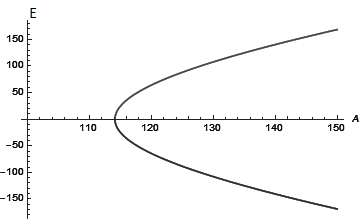
\includegraphics[scale=1]{imagenes/esp-energia.png}
    \caption{Energía del electrón en función del parámetro de energías del electrón A, $\epsilon=0.8$, $\gamma=0.64$, $\omega=100$}
    \label{fig:10.2}
\end{figure}

\begin{figure}[H]
    \centering
    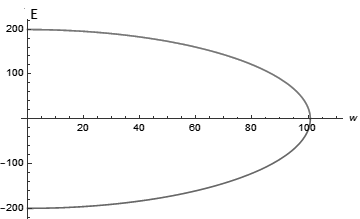
\includegraphics[scale=.8]{imagenes/ener-w.png}
    \caption{Energía del electrón en función de la frecuencia forzante $\omega$, $\epsilon=0.8$, $\gamma=0.64$, $A=115$}
    \label{fig:10.3}
\end{figure}

\begin{figure}[H]
    \centering
    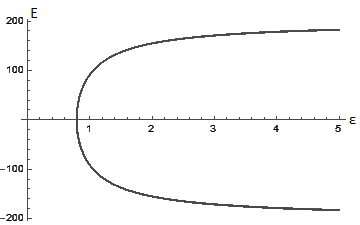
\includegraphics[scale=1]{imagenes/ener-e.png}
    \caption{Energía del electrón en función del parámetro $\epsilon$, $\omega=100$, $\gamma=0.64$, $A=115$}
    \label{fig:10.4}
\end{figure}

Se observa que la condición para estabilidad de las soluciones junto con la condición de no trivialidad ocasionan que la energía este limitada para ciertos valores de $A$, $\epsilon$ y $\omega$.

\subsection{Cálculo de las autofunciones}

Se calculan ahora las autofunciones del electrón, recordando las soluciones a las ecuaciones de Hill, se tiene que las soluciones de \ref{eq:10.40} tienen la forma:

\begin{equation}\label{eq:10.50}
    \psi(\rho)=\sum^{\infty}_{n=-\infty} b_n e^{i(an+\lambda)\rho}
\end{equation}

Además de la teoría de la expansión de Floquet-Magnus, las autofunciones del electrón estarán dadas por:

\begin{equation}\label{eq:10.51}
    \Psi(t,p)=P(t)e^{i\overline{H}t}\psi(p)
\end{equation}

Haciendo uso de \ref{eq:10.50} y \ref{eq:10.51} se obtiene la forma de la función de onda del electrón en el sistema.

\small
\begin{equation}\label{eq:10.52}
    \begin{split}
    &\Psi(\rho,t)=e^{-iEt}\sum^{\infty}_{n=-\infty}b_n\frac{e^{i \rho (a n+\lambda)}}{12 \omega^2} (-4 i (\omega (a n+\lambda) \sin (t \omega) \left(\gamma (a n+\lambda)^2-3 \epsilon\right)+\\&+4 a A \sin
   ^2\left(\frac{t \omega}{2}\right) \left(\sin (a \rho) \left(\gamma \left(3 a^2 n^2+a^2+6 a n \lambda+3 \lambda^2\right)-3 \epsilon\right)-3 i
   a \gamma (a n+\lambda) \cos (a \rho)\right))+\\&+\epsilon (a n+\lambda)^2 \cos (2 t \omega) \left(3 \epsilon-2 \gamma (a
   n+\lambda)^2\right)+\epsilon (a n+\lambda)^2 \left(2 \gamma (a n+\lambda)^2-3 \epsilon\right)+12 \omega^2)
   \end{split}
\end{equation}

\normalsize
Teniendo la forma de las autofunciones es posible hacer un estudio de la dinámica del electrón en el sistema de estudio y evaluar el comportamiento de las densidades de probabilidad en el espacio real y recíproco. De tal manera que es posible conocer la posición del electrón en el espacio de momentos y el espacio real para distintos espacios temporales. 

\begin{figure}[H]
    \centering
    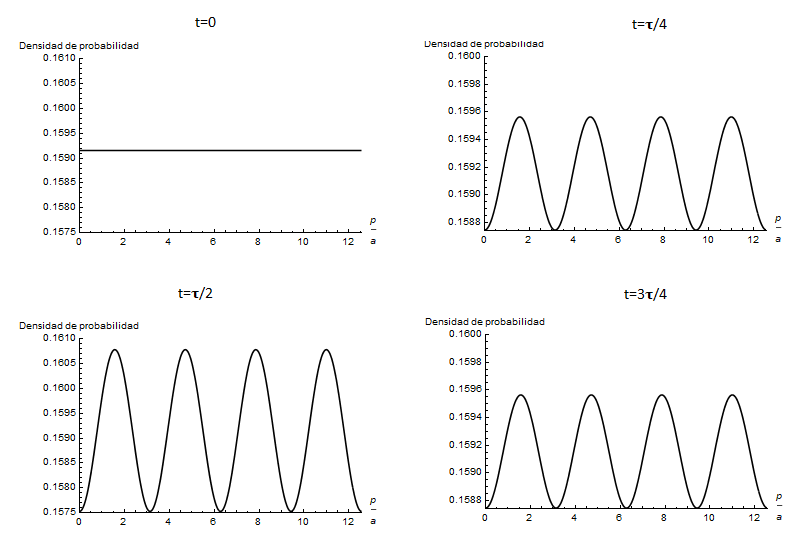
\includegraphics[width=1\columnwidth]{imagenes/dens_prop_pt0.png}
    \caption{Densidad de probabilidad en el espacio reciproco en función del momento en distintos $t$ que están dentro de un periodo de oscilación rápida $\tau=2\pi/\omega$, $\omega=50$, $a=0.1$, $A=1000$, $\epsilon=0.9$, $\gamma=0.81$}
    \label{fig5.11}
\end{figure}

Se observa que existe una periodicidad en el comportamiento de la densidad de probabilidad en el espacio de momentos $\rho$, con periodo $\tau=2\pi/\omega$. Durante este periodo la densidad de probabilidad pasa de tener una frecuencia nula a tener una frecuencia bien definida, con aumentos y disminución de la intensidad periódicos. Esto indica que en todo momento el electrón tiene una frecuencia de onda en el espacio recíproco constante, por lo que se espera que en el espacio real el electrón se encuentre bien localizado. 

\begin{figure}[H]
    \centering
    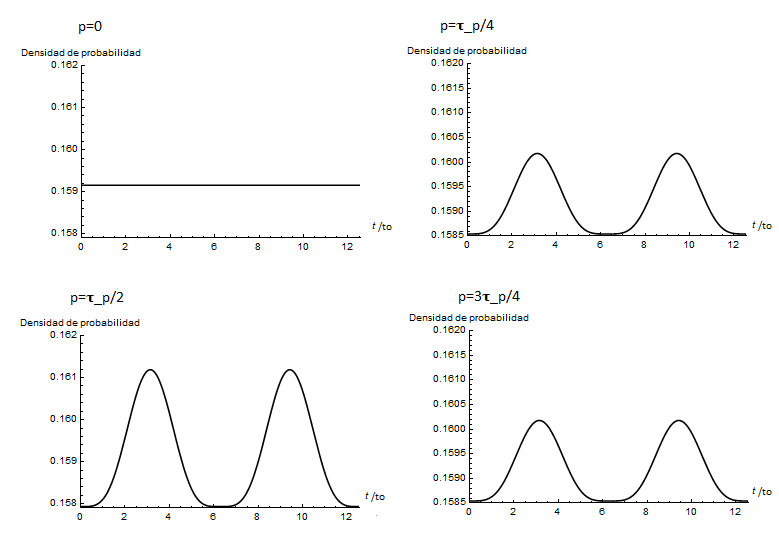
\includegraphics[width=1\columnwidth]{imagenes/dens_prop_tp1.png}
    \caption{Densidad de probabilidad en el espacio rec\'iproco en función del tiempo para distintos $\rho$ que están dentro de un periodo $\tau_{\rho}=2\pi/a$, $\omega=50$, $a=0.1$, $A=1000$, $\epsilon=0.9$, $\gamma=0.81$}
    \label{fig10.6}
\end{figure}

Una mirada al comportamiento de la densidad de probabilidad del electrón en el espacio recíproco en función del tiempo para distintos $\rho$, indica que para momento nulo o múltiplos de un periodo la densidad de probabilidad del electrón permanece constante, mientras que para momentos que están dentro del intervalo abierto $(0,2\pi/a)$  la densidad de probabilidad experimentará oscilaciones de frecuencia constante.  

Calculando la transformada de Fourier de la función de onda encontrada para el electrón, es posible obtener la expresión para la función de onda del electrón en el espacio real. A partir de ésta se halló la densidad de probabilidad y se han realizado los siguientes gráficos de densidad de probabilidad en el espacio real en distintos tiempos, para tiempos que están dentro del periodo $\tau=2\pi/\omega$. 

\begin{figure}[H]
    \centering
    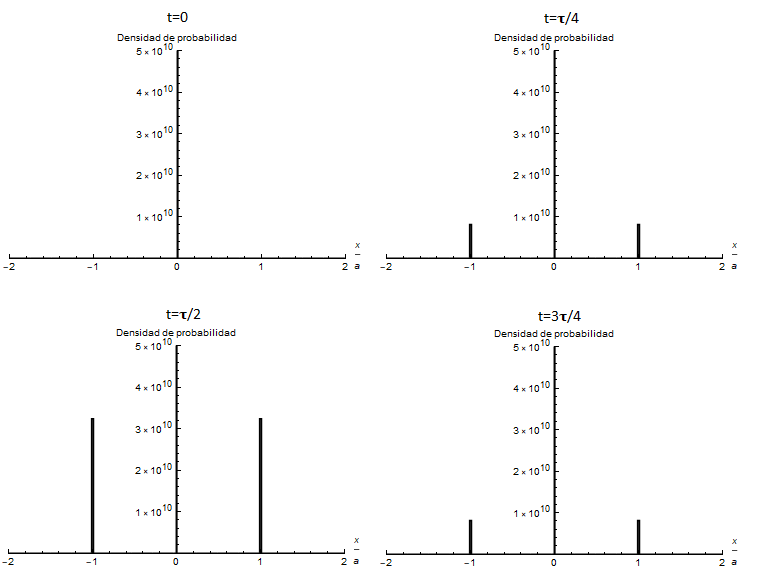
\includegraphics[width=1\columnwidth]{imagenes/dens_prop_tx.png}
    \caption{Densidad de probabilidad en el espacio real para distintos $t$, en un periodo $\tau=2\pi/\omega$, $\omega=50$, $a=0.1$, $A=1000$, $\epsilon=0.9$, $\gamma=0.81$}
    \label{fig5.13}
\end{figure}

Se encuentra que la posición del electrón en el espacio real se encuentra bien definida como deltas de Dirac. En $t=0$ o múltiplos del periodo, el electrón estará totalmente localizado en $x=0$, para tiempos intermedios el electrón tendrá tres posibles puntos de localización simétricos con el eje de las ordenadas. 

Una de las condiciones para afirmar la existencia de la localización dinámica del electrón, es que el valor esperado de la posición cuadrática esté acotada para todo tiempo. Al calcularlo se ha podido determinar que el valor esperado de la posición cuadrática es en efecto periódica y acotada para todo tiempo t. El siguiente gráfico muestra la forma resultante de la función que se obtuvo.

\begin{figure}[H]
    \centering
    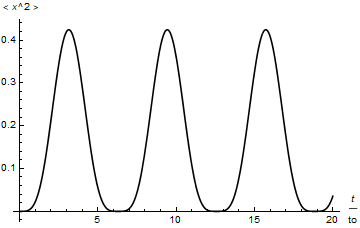
\includegraphics[scale=.7]{imagenes/x2-prom.png}
    \caption{Valor esperado de la posición al cuadrado en función del tiempo,$\omega=50$, $a=0.1$, $A=1000$, $\epsilon=0.9$, $\gamma=0.81$,$t_0=0,02$}
    \label{fig:5.14}
\end{figure}

De igual manera se ha calculado el valor esperado del momento cuadrado, se ha encontrado que este también es acotado y periódico, con valores que van desde cero asta un valor máximo, esto es evidencia de un comportamiento oscilatorio del electrón en el sistema de estudio. El siguiente gráfico muestra el comportamiento antes mencionado.

\begin{figure}[H]
    \centering
    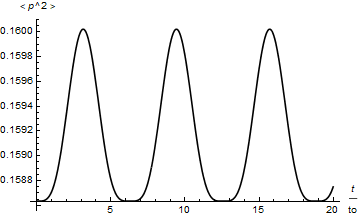
\includegraphics[scale=.7]{imagenes/p2-prom.png}
    \caption{Valor esperado del momentum al cuadrado en función del tiempo, $\omega=50$, $a=0.1$, $A=1000$, $\epsilon=0.9$, $\gamma=0.81$,$t_0=0,02$}
    \label{fig:5.15}
\end{figure}

Finalmente se ha calculado el valor esperado de momento y la posición del electrón, encontrándose que ambos tienen valor cero, lo cual confirma, junto con los otros resultados encontrados, que el electrón presenta el fenómeno de localización dinámica en el sistema de estudio.
\begin{equation}
    \begin{cases}
    \overline{x}=0\\ 
    \overline{p}=0
    \end{cases}
\end{equation}
